\documentclass{beamer}
\usepackage[T1]{fontenc}
\usepackage[french]{babel}
\usepackage{subfig}
\usepackage{tikz}
\usetikzlibrary{arrows}
\usepackage{pgf}

\usetheme{Madrid}
\usecolortheme{crane}
\useoutertheme{miniframes}
\useinnertheme{circles}

\definecolor{blendedblue}{rgb}{0.2,0.2,0.7}

\setbeamercolor{palette primary}{bg=blendedblue,fg=white}
\setbeamercolor{palette secondary}{bg=blendedblue,fg=white}
\setbeamercolor{palette tertiary}{bg=blendedblue,fg=white}
\setbeamercolor{palette quaternary}{bg=blendedblue,fg=white}
\setbeamercolor{structure}{fg=blendedblue} 
\setbeamercolor{section in toc}{fg=blendedblue}
\setbeamercolor{block title}{fg=white,bg=blendedblue}       
\setbeamercolor{block title example}{fg=white}
\setbeamercolor{block title alerted}{fg=white}
\setbeamercolor{subsection in head/foot}{bg=blendedblue!70,fg=white}

\title{Titre}
\author{Augustin Albert}

\begin{document}

\begin{frame}
	\titlepage
\end{frame}
\begin{frame}
	\centering{\large{Inserer la problematique}} 
	\tableofcontents
\end{frame}

\section{Détection des houppiers}

\begin{frame}
	Explication de la théorie: problème de detection de blob a multiples échelles : Théorie ... lindbergh
	\[G_{\sigma}:=\frac{1}{2\pi\sigma^{2}}\exp(-\frac{x^{2}+y^{2}}{2\sigma^{2}})\]
	\[{LoG}_{\sigma}:=-\frac{1}{\pi\sigma^{4}}(1-\frac{x^{2}+y^{2}}{2\sigma^{2}})\exp(-\frac{x^{2}+y^{2}}{2\sigma^{2}})\] 
	$\sigma=\frac{r}{\sqrt{2}}$
\end{frame}

\begin{frame}
	Paramètres du systeme et méthode heuristique -> possibilité d'avoir plusieurs arbre possible si suffisamment fin.
	$\sigma$, le nombre d'octave o et le nombre d'intervalle pour chaque octave i. La hauteur est $o \times i$ et le ratio $2^{\frac{1}{i}}$. 
\end{frame}

\begin{frame}
	\begin{figure}
		\subfloat[Réponse à une marche\label{fig:a}]{\scalebox{0.3}{%% Creator: Matplotlib, PGF backend
%%
%% To include the figure in your LaTeX document, write
%%   \input{<filename>.pgf}
%%
%% Make sure the required packages are loaded in your preamble
%%   \usepackage{pgf}
%%
%% Figures using additional raster images can only be included by \input if
%% they are in the same directory as the main LaTeX file. For loading figures
%% from other directories you can use the `import` package
%%   \usepackage{import}
%%
%% and then include the figures with
%%   \import{<path to file>}{<filename>.pgf}
%%
%% Matplotlib used the following preamble
%%   \usepackage{fontspec}
%%   \setmainfont{DejaVuSerif.ttf}[Path=\detokenize{/home/aalbert/.local/lib/python3.9/site-packages/matplotlib/mpl-data/fonts/ttf/}]
%%   \setsansfont{DejaVuSans.ttf}[Path=\detokenize{/home/aalbert/.local/lib/python3.9/site-packages/matplotlib/mpl-data/fonts/ttf/}]
%%   \setmonofont{DejaVuSansMono.ttf}[Path=\detokenize{/home/aalbert/.local/lib/python3.9/site-packages/matplotlib/mpl-data/fonts/ttf/}]
%%
\begingroup%
\makeatletter%
\begin{pgfpicture}%
\pgfpathrectangle{\pgfpointorigin}{\pgfqpoint{6.400000in}{4.800000in}}%
\pgfusepath{use as bounding box, clip}%
\begin{pgfscope}%
\pgfsetbuttcap%
\pgfsetmiterjoin%
\definecolor{currentfill}{rgb}{1.000000,1.000000,1.000000}%
\pgfsetfillcolor{currentfill}%
\pgfsetlinewidth{0.000000pt}%
\definecolor{currentstroke}{rgb}{1.000000,1.000000,1.000000}%
\pgfsetstrokecolor{currentstroke}%
\pgfsetdash{}{0pt}%
\pgfpathmoveto{\pgfqpoint{0.000000in}{0.000000in}}%
\pgfpathlineto{\pgfqpoint{6.400000in}{0.000000in}}%
\pgfpathlineto{\pgfqpoint{6.400000in}{4.800000in}}%
\pgfpathlineto{\pgfqpoint{0.000000in}{4.800000in}}%
\pgfpathclose%
\pgfusepath{fill}%
\end{pgfscope}%
\begin{pgfscope}%
\pgfpathrectangle{\pgfqpoint{0.800000in}{0.528000in}}{\pgfqpoint{4.960000in}{3.696000in}}%
\pgfusepath{clip}%
\pgfsetrectcap%
\pgfsetroundjoin%
\pgfsetlinewidth{4.015000pt}%
\definecolor{currentstroke}{rgb}{0.121569,0.466667,0.705882}%
\pgfsetstrokecolor{currentstroke}%
\pgfsetdash{}{0pt}%
\pgfpathmoveto{\pgfqpoint{1.025455in}{2.373256in}}%
\pgfpathlineto{\pgfqpoint{3.268671in}{2.373256in}}%
\pgfpathlineto{\pgfqpoint{3.291329in}{4.056000in}}%
\pgfpathlineto{\pgfqpoint{5.534545in}{4.056000in}}%
\pgfpathlineto{\pgfqpoint{5.534545in}{4.056000in}}%
\pgfusepath{stroke}%
\end{pgfscope}%
\begin{pgfscope}%
\pgfpathrectangle{\pgfqpoint{0.800000in}{0.528000in}}{\pgfqpoint{4.960000in}{3.696000in}}%
\pgfusepath{clip}%
\pgfsetrectcap%
\pgfsetroundjoin%
\pgfsetlinewidth{4.015000pt}%
\definecolor{currentstroke}{rgb}{1.000000,0.498039,0.054902}%
\pgfsetstrokecolor{currentstroke}%
\pgfsetdash{}{0pt}%
\pgfpathmoveto{\pgfqpoint{1.025455in}{2.373256in}}%
\pgfpathlineto{\pgfqpoint{2.045098in}{2.372178in}}%
\pgfpathlineto{\pgfqpoint{2.135733in}{2.370208in}}%
\pgfpathlineto{\pgfqpoint{2.203709in}{2.366947in}}%
\pgfpathlineto{\pgfqpoint{2.249027in}{2.363259in}}%
\pgfpathlineto{\pgfqpoint{2.294344in}{2.357726in}}%
\pgfpathlineto{\pgfqpoint{2.339662in}{2.349603in}}%
\pgfpathlineto{\pgfqpoint{2.384979in}{2.337938in}}%
\pgfpathlineto{\pgfqpoint{2.407638in}{2.330418in}}%
\pgfpathlineto{\pgfqpoint{2.430297in}{2.321554in}}%
\pgfpathlineto{\pgfqpoint{2.452956in}{2.311163in}}%
\pgfpathlineto{\pgfqpoint{2.475614in}{2.299053in}}%
\pgfpathlineto{\pgfqpoint{2.498273in}{2.285018in}}%
\pgfpathlineto{\pgfqpoint{2.520932in}{2.268847in}}%
\pgfpathlineto{\pgfqpoint{2.543591in}{2.250322in}}%
\pgfpathlineto{\pgfqpoint{2.566249in}{2.229225in}}%
\pgfpathlineto{\pgfqpoint{2.588908in}{2.205341in}}%
\pgfpathlineto{\pgfqpoint{2.611567in}{2.178463in}}%
\pgfpathlineto{\pgfqpoint{2.634226in}{2.148398in}}%
\pgfpathlineto{\pgfqpoint{2.656884in}{2.114974in}}%
\pgfpathlineto{\pgfqpoint{2.679543in}{2.078047in}}%
\pgfpathlineto{\pgfqpoint{2.702202in}{2.037505in}}%
\pgfpathlineto{\pgfqpoint{2.724861in}{1.993282in}}%
\pgfpathlineto{\pgfqpoint{2.747519in}{1.945357in}}%
\pgfpathlineto{\pgfqpoint{2.770178in}{1.893766in}}%
\pgfpathlineto{\pgfqpoint{2.792837in}{1.838607in}}%
\pgfpathlineto{\pgfqpoint{2.815496in}{1.780047in}}%
\pgfpathlineto{\pgfqpoint{2.860813in}{1.653745in}}%
\pgfpathlineto{\pgfqpoint{2.906131in}{1.517659in}}%
\pgfpathlineto{\pgfqpoint{3.042083in}{1.095707in}}%
\pgfpathlineto{\pgfqpoint{3.064742in}{1.030885in}}%
\pgfpathlineto{\pgfqpoint{3.087401in}{0.969738in}}%
\pgfpathlineto{\pgfqpoint{3.110059in}{0.913051in}}%
\pgfpathlineto{\pgfqpoint{3.132718in}{0.861575in}}%
\pgfpathlineto{\pgfqpoint{3.155377in}{0.816010in}}%
\pgfpathlineto{\pgfqpoint{3.178036in}{0.776993in}}%
\pgfpathlineto{\pgfqpoint{3.200694in}{0.745076in}}%
\pgfpathlineto{\pgfqpoint{3.223353in}{0.720720in}}%
\pgfpathlineto{\pgfqpoint{3.246012in}{0.704281in}}%
\pgfpathlineto{\pgfqpoint{3.268671in}{0.696000in}}%
\pgfpathlineto{\pgfqpoint{3.291329in}{0.696000in}}%
\pgfpathlineto{\pgfqpoint{3.313988in}{0.704281in}}%
\pgfpathlineto{\pgfqpoint{3.336647in}{0.720720in}}%
\pgfpathlineto{\pgfqpoint{3.359306in}{0.745076in}}%
\pgfpathlineto{\pgfqpoint{3.381964in}{0.776993in}}%
\pgfpathlineto{\pgfqpoint{3.404623in}{0.816010in}}%
\pgfpathlineto{\pgfqpoint{3.427282in}{0.861575in}}%
\pgfpathlineto{\pgfqpoint{3.449941in}{0.913051in}}%
\pgfpathlineto{\pgfqpoint{3.472599in}{0.969738in}}%
\pgfpathlineto{\pgfqpoint{3.495258in}{1.030885in}}%
\pgfpathlineto{\pgfqpoint{3.540576in}{1.163401in}}%
\pgfpathlineto{\pgfqpoint{3.608552in}{1.375778in}}%
\pgfpathlineto{\pgfqpoint{3.676528in}{1.586703in}}%
\pgfpathlineto{\pgfqpoint{3.721846in}{1.718322in}}%
\pgfpathlineto{\pgfqpoint{3.767163in}{1.838607in}}%
\pgfpathlineto{\pgfqpoint{3.789822in}{1.893766in}}%
\pgfpathlineto{\pgfqpoint{3.812481in}{1.945357in}}%
\pgfpathlineto{\pgfqpoint{3.835139in}{1.993282in}}%
\pgfpathlineto{\pgfqpoint{3.857798in}{2.037505in}}%
\pgfpathlineto{\pgfqpoint{3.880457in}{2.078047in}}%
\pgfpathlineto{\pgfqpoint{3.903116in}{2.114974in}}%
\pgfpathlineto{\pgfqpoint{3.925774in}{2.148398in}}%
\pgfpathlineto{\pgfqpoint{3.948433in}{2.178463in}}%
\pgfpathlineto{\pgfqpoint{3.971092in}{2.205341in}}%
\pgfpathlineto{\pgfqpoint{3.993751in}{2.229225in}}%
\pgfpathlineto{\pgfqpoint{4.016409in}{2.250322in}}%
\pgfpathlineto{\pgfqpoint{4.039068in}{2.268847in}}%
\pgfpathlineto{\pgfqpoint{4.061727in}{2.285018in}}%
\pgfpathlineto{\pgfqpoint{4.084386in}{2.299053in}}%
\pgfpathlineto{\pgfqpoint{4.107044in}{2.311163in}}%
\pgfpathlineto{\pgfqpoint{4.129703in}{2.321554in}}%
\pgfpathlineto{\pgfqpoint{4.152362in}{2.330418in}}%
\pgfpathlineto{\pgfqpoint{4.175021in}{2.337938in}}%
\pgfpathlineto{\pgfqpoint{4.220338in}{2.349603in}}%
\pgfpathlineto{\pgfqpoint{4.265656in}{2.357726in}}%
\pgfpathlineto{\pgfqpoint{4.310973in}{2.363259in}}%
\pgfpathlineto{\pgfqpoint{4.378949in}{2.368281in}}%
\pgfpathlineto{\pgfqpoint{4.446926in}{2.370888in}}%
\pgfpathlineto{\pgfqpoint{4.560219in}{2.372634in}}%
\pgfpathlineto{\pgfqpoint{4.809466in}{2.373235in}}%
\pgfpathlineto{\pgfqpoint{5.534545in}{2.373256in}}%
\pgfpathlineto{\pgfqpoint{5.534545in}{2.373256in}}%
\pgfusepath{stroke}%
\end{pgfscope}%
\end{pgfpicture}%
\makeatother%
\endgroup%
}}
		\subfloat[Réponse à un créneau pour $\sigma=1$, $\sigma=2$ et $\sigma=3$ \label{fig:b}]{\scalebox{0.3}{%% Creator: Matplotlib, PGF backend
%%
%% To include the figure in your LaTeX document, write
%%   \input{<filename>.pgf}
%%
%% Make sure the required packages are loaded in your preamble
%%   \usepackage{pgf}
%%
%% Figures using additional raster images can only be included by \input if
%% they are in the same directory as the main LaTeX file. For loading figures
%% from other directories you can use the `import` package
%%   \usepackage{import}
%%
%% and then include the figures with
%%   \import{<path to file>}{<filename>.pgf}
%%
%% Matplotlib used the following preamble
%%   \usepackage{fontspec}
%%   \setmainfont{DejaVuSerif.ttf}[Path=\detokenize{/home/aalbert/.local/lib/python3.9/site-packages/matplotlib/mpl-data/fonts/ttf/}]
%%   \setsansfont{DejaVuSans.ttf}[Path=\detokenize{/home/aalbert/.local/lib/python3.9/site-packages/matplotlib/mpl-data/fonts/ttf/}]
%%   \setmonofont{DejaVuSansMono.ttf}[Path=\detokenize{/home/aalbert/.local/lib/python3.9/site-packages/matplotlib/mpl-data/fonts/ttf/}]
%%
\begingroup%
\makeatletter%
\begin{pgfpicture}%
\pgfpathrectangle{\pgfpointorigin}{\pgfqpoint{6.400000in}{4.800000in}}%
\pgfusepath{use as bounding box, clip}%
\begin{pgfscope}%
\pgfsetbuttcap%
\pgfsetmiterjoin%
\definecolor{currentfill}{rgb}{1.000000,1.000000,1.000000}%
\pgfsetfillcolor{currentfill}%
\pgfsetlinewidth{0.000000pt}%
\definecolor{currentstroke}{rgb}{1.000000,1.000000,1.000000}%
\pgfsetstrokecolor{currentstroke}%
\pgfsetdash{}{0pt}%
\pgfpathmoveto{\pgfqpoint{0.000000in}{0.000000in}}%
\pgfpathlineto{\pgfqpoint{6.400000in}{0.000000in}}%
\pgfpathlineto{\pgfqpoint{6.400000in}{4.800000in}}%
\pgfpathlineto{\pgfqpoint{0.000000in}{4.800000in}}%
\pgfpathclose%
\pgfusepath{fill}%
\end{pgfscope}%
\begin{pgfscope}%
\pgfpathrectangle{\pgfqpoint{0.800000in}{0.528000in}}{\pgfqpoint{4.960000in}{3.696000in}}%
\pgfusepath{clip}%
\pgfsetrectcap%
\pgfsetroundjoin%
\pgfsetlinewidth{4.015000pt}%
\definecolor{currentstroke}{rgb}{0.121569,0.466667,0.705882}%
\pgfsetstrokecolor{currentstroke}%
\pgfsetdash{}{0pt}%
\pgfpathmoveto{\pgfqpoint{1.025455in}{2.582780in}}%
\pgfpathlineto{\pgfqpoint{2.702202in}{2.582780in}}%
\pgfpathlineto{\pgfqpoint{2.724861in}{4.056000in}}%
\pgfpathlineto{\pgfqpoint{3.835139in}{4.056000in}}%
\pgfpathlineto{\pgfqpoint{3.857798in}{2.582780in}}%
\pgfpathlineto{\pgfqpoint{5.534545in}{2.582780in}}%
\pgfpathlineto{\pgfqpoint{5.534545in}{2.582780in}}%
\pgfusepath{stroke}%
\end{pgfscope}%
\begin{pgfscope}%
\pgfpathrectangle{\pgfqpoint{0.800000in}{0.528000in}}{\pgfqpoint{4.960000in}{3.696000in}}%
\pgfusepath{clip}%
\pgfsetrectcap%
\pgfsetroundjoin%
\pgfsetlinewidth{4.015000pt}%
\definecolor{currentstroke}{rgb}{1.000000,0.498039,0.054902}%
\pgfsetstrokecolor{currentstroke}%
\pgfsetdash{}{0pt}%
\pgfpathmoveto{\pgfqpoint{1.025455in}{2.583098in}}%
\pgfpathlineto{\pgfqpoint{1.184066in}{2.584561in}}%
\pgfpathlineto{\pgfqpoint{1.274701in}{2.587159in}}%
\pgfpathlineto{\pgfqpoint{1.342677in}{2.591035in}}%
\pgfpathlineto{\pgfqpoint{1.387995in}{2.595134in}}%
\pgfpathlineto{\pgfqpoint{1.433312in}{2.600980in}}%
\pgfpathlineto{\pgfqpoint{1.478630in}{2.609173in}}%
\pgfpathlineto{\pgfqpoint{1.523947in}{2.620451in}}%
\pgfpathlineto{\pgfqpoint{1.569265in}{2.635696in}}%
\pgfpathlineto{\pgfqpoint{1.591923in}{2.645119in}}%
\pgfpathlineto{\pgfqpoint{1.614582in}{2.655925in}}%
\pgfpathlineto{\pgfqpoint{1.637241in}{2.668256in}}%
\pgfpathlineto{\pgfqpoint{1.659899in}{2.682260in}}%
\pgfpathlineto{\pgfqpoint{1.682558in}{2.698085in}}%
\pgfpathlineto{\pgfqpoint{1.705217in}{2.715880in}}%
\pgfpathlineto{\pgfqpoint{1.727876in}{2.735788in}}%
\pgfpathlineto{\pgfqpoint{1.750534in}{2.757944in}}%
\pgfpathlineto{\pgfqpoint{1.773193in}{2.782473in}}%
\pgfpathlineto{\pgfqpoint{1.795852in}{2.809481in}}%
\pgfpathlineto{\pgfqpoint{1.818511in}{2.839054in}}%
\pgfpathlineto{\pgfqpoint{1.841169in}{2.871254in}}%
\pgfpathlineto{\pgfqpoint{1.863828in}{2.906107in}}%
\pgfpathlineto{\pgfqpoint{1.886487in}{2.943604in}}%
\pgfpathlineto{\pgfqpoint{1.909146in}{2.983695in}}%
\pgfpathlineto{\pgfqpoint{1.954463in}{3.071206in}}%
\pgfpathlineto{\pgfqpoint{1.999781in}{3.167191in}}%
\pgfpathlineto{\pgfqpoint{2.045098in}{3.269236in}}%
\pgfpathlineto{\pgfqpoint{2.135733in}{3.476752in}}%
\pgfpathlineto{\pgfqpoint{2.181051in}{3.572437in}}%
\pgfpathlineto{\pgfqpoint{2.203709in}{3.615736in}}%
\pgfpathlineto{\pgfqpoint{2.226368in}{3.654958in}}%
\pgfpathlineto{\pgfqpoint{2.249027in}{3.689304in}}%
\pgfpathlineto{\pgfqpoint{2.271686in}{3.717980in}}%
\pgfpathlineto{\pgfqpoint{2.294344in}{3.740214in}}%
\pgfpathlineto{\pgfqpoint{2.317003in}{3.755268in}}%
\pgfpathlineto{\pgfqpoint{2.339662in}{3.762458in}}%
\pgfpathlineto{\pgfqpoint{2.362321in}{3.761169in}}%
\pgfpathlineto{\pgfqpoint{2.384979in}{3.750867in}}%
\pgfpathlineto{\pgfqpoint{2.407638in}{3.731120in}}%
\pgfpathlineto{\pgfqpoint{2.430297in}{3.701604in}}%
\pgfpathlineto{\pgfqpoint{2.452956in}{3.662118in}}%
\pgfpathlineto{\pgfqpoint{2.475614in}{3.612595in}}%
\pgfpathlineto{\pgfqpoint{2.498273in}{3.553101in}}%
\pgfpathlineto{\pgfqpoint{2.520932in}{3.483845in}}%
\pgfpathlineto{\pgfqpoint{2.543591in}{3.405179in}}%
\pgfpathlineto{\pgfqpoint{2.566249in}{3.317590in}}%
\pgfpathlineto{\pgfqpoint{2.588908in}{3.221699in}}%
\pgfpathlineto{\pgfqpoint{2.611567in}{3.118249in}}%
\pgfpathlineto{\pgfqpoint{2.634226in}{3.008093in}}%
\pgfpathlineto{\pgfqpoint{2.679543in}{2.771538in}}%
\pgfpathlineto{\pgfqpoint{2.724861in}{2.520441in}}%
\pgfpathlineto{\pgfqpoint{2.815496in}{2.010569in}}%
\pgfpathlineto{\pgfqpoint{2.860813in}{1.768893in}}%
\pgfpathlineto{\pgfqpoint{2.906131in}{1.545663in}}%
\pgfpathlineto{\pgfqpoint{2.928789in}{1.442658in}}%
\pgfpathlineto{\pgfqpoint{2.951448in}{1.346064in}}%
\pgfpathlineto{\pgfqpoint{2.974107in}{1.256232in}}%
\pgfpathlineto{\pgfqpoint{2.996766in}{1.173400in}}%
\pgfpathlineto{\pgfqpoint{3.019424in}{1.097692in}}%
\pgfpathlineto{\pgfqpoint{3.042083in}{1.029133in}}%
\pgfpathlineto{\pgfqpoint{3.064742in}{0.967657in}}%
\pgfpathlineto{\pgfqpoint{3.087401in}{0.913125in}}%
\pgfpathlineto{\pgfqpoint{3.110059in}{0.865338in}}%
\pgfpathlineto{\pgfqpoint{3.132718in}{0.824054in}}%
\pgfpathlineto{\pgfqpoint{3.155377in}{0.789010in}}%
\pgfpathlineto{\pgfqpoint{3.178036in}{0.759932in}}%
\pgfpathlineto{\pgfqpoint{3.200694in}{0.736559in}}%
\pgfpathlineto{\pgfqpoint{3.223353in}{0.718654in}}%
\pgfpathlineto{\pgfqpoint{3.246012in}{0.706016in}}%
\pgfpathlineto{\pgfqpoint{3.268671in}{0.698496in}}%
\pgfpathlineto{\pgfqpoint{3.291329in}{0.696000in}}%
\pgfpathlineto{\pgfqpoint{3.313988in}{0.698496in}}%
\pgfpathlineto{\pgfqpoint{3.336647in}{0.706016in}}%
\pgfpathlineto{\pgfqpoint{3.359306in}{0.718654in}}%
\pgfpathlineto{\pgfqpoint{3.381964in}{0.736559in}}%
\pgfpathlineto{\pgfqpoint{3.404623in}{0.759932in}}%
\pgfpathlineto{\pgfqpoint{3.427282in}{0.789010in}}%
\pgfpathlineto{\pgfqpoint{3.449941in}{0.824054in}}%
\pgfpathlineto{\pgfqpoint{3.472599in}{0.865338in}}%
\pgfpathlineto{\pgfqpoint{3.495258in}{0.913125in}}%
\pgfpathlineto{\pgfqpoint{3.517917in}{0.967657in}}%
\pgfpathlineto{\pgfqpoint{3.540576in}{1.029133in}}%
\pgfpathlineto{\pgfqpoint{3.563234in}{1.097692in}}%
\pgfpathlineto{\pgfqpoint{3.585893in}{1.173400in}}%
\pgfpathlineto{\pgfqpoint{3.608552in}{1.256232in}}%
\pgfpathlineto{\pgfqpoint{3.631211in}{1.346064in}}%
\pgfpathlineto{\pgfqpoint{3.653869in}{1.442658in}}%
\pgfpathlineto{\pgfqpoint{3.676528in}{1.545663in}}%
\pgfpathlineto{\pgfqpoint{3.721846in}{1.768893in}}%
\pgfpathlineto{\pgfqpoint{3.767163in}{2.010569in}}%
\pgfpathlineto{\pgfqpoint{3.835139in}{2.392250in}}%
\pgfpathlineto{\pgfqpoint{3.903116in}{2.771538in}}%
\pgfpathlineto{\pgfqpoint{3.948433in}{3.008093in}}%
\pgfpathlineto{\pgfqpoint{3.971092in}{3.118249in}}%
\pgfpathlineto{\pgfqpoint{3.993751in}{3.221699in}}%
\pgfpathlineto{\pgfqpoint{4.016409in}{3.317590in}}%
\pgfpathlineto{\pgfqpoint{4.039068in}{3.405179in}}%
\pgfpathlineto{\pgfqpoint{4.061727in}{3.483845in}}%
\pgfpathlineto{\pgfqpoint{4.084386in}{3.553101in}}%
\pgfpathlineto{\pgfqpoint{4.107044in}{3.612595in}}%
\pgfpathlineto{\pgfqpoint{4.129703in}{3.662118in}}%
\pgfpathlineto{\pgfqpoint{4.152362in}{3.701604in}}%
\pgfpathlineto{\pgfqpoint{4.175021in}{3.731120in}}%
\pgfpathlineto{\pgfqpoint{4.197679in}{3.750867in}}%
\pgfpathlineto{\pgfqpoint{4.220338in}{3.761169in}}%
\pgfpathlineto{\pgfqpoint{4.242997in}{3.762458in}}%
\pgfpathlineto{\pgfqpoint{4.265656in}{3.755268in}}%
\pgfpathlineto{\pgfqpoint{4.288314in}{3.740214in}}%
\pgfpathlineto{\pgfqpoint{4.310973in}{3.717980in}}%
\pgfpathlineto{\pgfqpoint{4.333632in}{3.689304in}}%
\pgfpathlineto{\pgfqpoint{4.356291in}{3.654958in}}%
\pgfpathlineto{\pgfqpoint{4.378949in}{3.615736in}}%
\pgfpathlineto{\pgfqpoint{4.401608in}{3.572437in}}%
\pgfpathlineto{\pgfqpoint{4.446926in}{3.476752in}}%
\pgfpathlineto{\pgfqpoint{4.514902in}{3.321498in}}%
\pgfpathlineto{\pgfqpoint{4.582878in}{3.167191in}}%
\pgfpathlineto{\pgfqpoint{4.628196in}{3.071206in}}%
\pgfpathlineto{\pgfqpoint{4.673513in}{2.983695in}}%
\pgfpathlineto{\pgfqpoint{4.696172in}{2.943604in}}%
\pgfpathlineto{\pgfqpoint{4.718831in}{2.906107in}}%
\pgfpathlineto{\pgfqpoint{4.741489in}{2.871254in}}%
\pgfpathlineto{\pgfqpoint{4.764148in}{2.839054in}}%
\pgfpathlineto{\pgfqpoint{4.786807in}{2.809481in}}%
\pgfpathlineto{\pgfqpoint{4.809466in}{2.782473in}}%
\pgfpathlineto{\pgfqpoint{4.832124in}{2.757944in}}%
\pgfpathlineto{\pgfqpoint{4.854783in}{2.735788in}}%
\pgfpathlineto{\pgfqpoint{4.877442in}{2.715880in}}%
\pgfpathlineto{\pgfqpoint{4.900101in}{2.698085in}}%
\pgfpathlineto{\pgfqpoint{4.922759in}{2.682260in}}%
\pgfpathlineto{\pgfqpoint{4.945418in}{2.668256in}}%
\pgfpathlineto{\pgfqpoint{4.968077in}{2.655925in}}%
\pgfpathlineto{\pgfqpoint{4.990735in}{2.645119in}}%
\pgfpathlineto{\pgfqpoint{5.013394in}{2.635696in}}%
\pgfpathlineto{\pgfqpoint{5.058712in}{2.620451in}}%
\pgfpathlineto{\pgfqpoint{5.104029in}{2.609173in}}%
\pgfpathlineto{\pgfqpoint{5.149347in}{2.600980in}}%
\pgfpathlineto{\pgfqpoint{5.194664in}{2.595134in}}%
\pgfpathlineto{\pgfqpoint{5.262640in}{2.589489in}}%
\pgfpathlineto{\pgfqpoint{5.330617in}{2.586298in}}%
\pgfpathlineto{\pgfqpoint{5.443910in}{2.583890in}}%
\pgfpathlineto{\pgfqpoint{5.534545in}{2.583192in}}%
\pgfpathlineto{\pgfqpoint{5.534545in}{2.583192in}}%
\pgfusepath{stroke}%
\end{pgfscope}%
\begin{pgfscope}%
\pgfpathrectangle{\pgfqpoint{0.800000in}{0.528000in}}{\pgfqpoint{4.960000in}{3.696000in}}%
\pgfusepath{clip}%
\pgfsetrectcap%
\pgfsetroundjoin%
\pgfsetlinewidth{4.015000pt}%
\definecolor{currentstroke}{rgb}{0.172549,0.627451,0.172549}%
\pgfsetstrokecolor{currentstroke}%
\pgfsetdash{}{0pt}%
\pgfpathmoveto{\pgfqpoint{1.025455in}{2.588651in}}%
\pgfpathlineto{\pgfqpoint{1.138748in}{2.593352in}}%
\pgfpathlineto{\pgfqpoint{1.229383in}{2.598995in}}%
\pgfpathlineto{\pgfqpoint{1.320018in}{2.606737in}}%
\pgfpathlineto{\pgfqpoint{1.410653in}{2.616866in}}%
\pgfpathlineto{\pgfqpoint{1.501288in}{2.629427in}}%
\pgfpathlineto{\pgfqpoint{1.614582in}{2.647921in}}%
\pgfpathlineto{\pgfqpoint{1.795852in}{2.678071in}}%
\pgfpathlineto{\pgfqpoint{1.863828in}{2.686567in}}%
\pgfpathlineto{\pgfqpoint{1.909146in}{2.690337in}}%
\pgfpathlineto{\pgfqpoint{1.954463in}{2.692055in}}%
\pgfpathlineto{\pgfqpoint{1.999781in}{2.691231in}}%
\pgfpathlineto{\pgfqpoint{2.045098in}{2.687365in}}%
\pgfpathlineto{\pgfqpoint{2.090416in}{2.679963in}}%
\pgfpathlineto{\pgfqpoint{2.135733in}{2.668555in}}%
\pgfpathlineto{\pgfqpoint{2.181051in}{2.652709in}}%
\pgfpathlineto{\pgfqpoint{2.203709in}{2.643005in}}%
\pgfpathlineto{\pgfqpoint{2.226368in}{2.632060in}}%
\pgfpathlineto{\pgfqpoint{2.249027in}{2.619840in}}%
\pgfpathlineto{\pgfqpoint{2.271686in}{2.606319in}}%
\pgfpathlineto{\pgfqpoint{2.294344in}{2.591476in}}%
\pgfpathlineto{\pgfqpoint{2.339662in}{2.557778in}}%
\pgfpathlineto{\pgfqpoint{2.384979in}{2.518732in}}%
\pgfpathlineto{\pgfqpoint{2.430297in}{2.474457in}}%
\pgfpathlineto{\pgfqpoint{2.475614in}{2.425206in}}%
\pgfpathlineto{\pgfqpoint{2.520932in}{2.371372in}}%
\pgfpathlineto{\pgfqpoint{2.566249in}{2.313485in}}%
\pgfpathlineto{\pgfqpoint{2.611567in}{2.252203in}}%
\pgfpathlineto{\pgfqpoint{2.679543in}{2.155634in}}%
\pgfpathlineto{\pgfqpoint{2.860813in}{1.893297in}}%
\pgfpathlineto{\pgfqpoint{2.906131in}{1.832169in}}%
\pgfpathlineto{\pgfqpoint{2.951448in}{1.774885in}}%
\pgfpathlineto{\pgfqpoint{2.996766in}{1.722410in}}%
\pgfpathlineto{\pgfqpoint{3.042083in}{1.675635in}}%
\pgfpathlineto{\pgfqpoint{3.064742in}{1.654640in}}%
\pgfpathlineto{\pgfqpoint{3.087401in}{1.635361in}}%
\pgfpathlineto{\pgfqpoint{3.110059in}{1.617882in}}%
\pgfpathlineto{\pgfqpoint{3.132718in}{1.602277in}}%
\pgfpathlineto{\pgfqpoint{3.155377in}{1.588615in}}%
\pgfpathlineto{\pgfqpoint{3.178036in}{1.576953in}}%
\pgfpathlineto{\pgfqpoint{3.200694in}{1.567342in}}%
\pgfpathlineto{\pgfqpoint{3.223353in}{1.559824in}}%
\pgfpathlineto{\pgfqpoint{3.246012in}{1.554430in}}%
\pgfpathlineto{\pgfqpoint{3.268671in}{1.551185in}}%
\pgfpathlineto{\pgfqpoint{3.291329in}{1.550102in}}%
\pgfpathlineto{\pgfqpoint{3.313988in}{1.551185in}}%
\pgfpathlineto{\pgfqpoint{3.336647in}{1.554430in}}%
\pgfpathlineto{\pgfqpoint{3.359306in}{1.559824in}}%
\pgfpathlineto{\pgfqpoint{3.381964in}{1.567342in}}%
\pgfpathlineto{\pgfqpoint{3.404623in}{1.576953in}}%
\pgfpathlineto{\pgfqpoint{3.427282in}{1.588615in}}%
\pgfpathlineto{\pgfqpoint{3.449941in}{1.602277in}}%
\pgfpathlineto{\pgfqpoint{3.472599in}{1.617882in}}%
\pgfpathlineto{\pgfqpoint{3.495258in}{1.635361in}}%
\pgfpathlineto{\pgfqpoint{3.517917in}{1.654640in}}%
\pgfpathlineto{\pgfqpoint{3.540576in}{1.675635in}}%
\pgfpathlineto{\pgfqpoint{3.585893in}{1.722410in}}%
\pgfpathlineto{\pgfqpoint{3.631211in}{1.774885in}}%
\pgfpathlineto{\pgfqpoint{3.676528in}{1.832169in}}%
\pgfpathlineto{\pgfqpoint{3.721846in}{1.893297in}}%
\pgfpathlineto{\pgfqpoint{3.789822in}{1.989965in}}%
\pgfpathlineto{\pgfqpoint{3.948433in}{2.220527in}}%
\pgfpathlineto{\pgfqpoint{3.993751in}{2.283223in}}%
\pgfpathlineto{\pgfqpoint{4.039068in}{2.342897in}}%
\pgfpathlineto{\pgfqpoint{4.084386in}{2.398832in}}%
\pgfpathlineto{\pgfqpoint{4.129703in}{2.450432in}}%
\pgfpathlineto{\pgfqpoint{4.175021in}{2.497236in}}%
\pgfpathlineto{\pgfqpoint{4.220338in}{2.538919in}}%
\pgfpathlineto{\pgfqpoint{4.265656in}{2.575297in}}%
\pgfpathlineto{\pgfqpoint{4.310973in}{2.606319in}}%
\pgfpathlineto{\pgfqpoint{4.333632in}{2.619840in}}%
\pgfpathlineto{\pgfqpoint{4.356291in}{2.632060in}}%
\pgfpathlineto{\pgfqpoint{4.378949in}{2.643005in}}%
\pgfpathlineto{\pgfqpoint{4.424267in}{2.661211in}}%
\pgfpathlineto{\pgfqpoint{4.469584in}{2.674788in}}%
\pgfpathlineto{\pgfqpoint{4.514902in}{2.684136in}}%
\pgfpathlineto{\pgfqpoint{4.560219in}{2.689709in}}%
\pgfpathlineto{\pgfqpoint{4.605537in}{2.691992in}}%
\pgfpathlineto{\pgfqpoint{4.650854in}{2.691483in}}%
\pgfpathlineto{\pgfqpoint{4.696172in}{2.688679in}}%
\pgfpathlineto{\pgfqpoint{4.741489in}{2.684059in}}%
\pgfpathlineto{\pgfqpoint{4.809466in}{2.674694in}}%
\pgfpathlineto{\pgfqpoint{4.922759in}{2.655762in}}%
\pgfpathlineto{\pgfqpoint{5.058712in}{2.632917in}}%
\pgfpathlineto{\pgfqpoint{5.149347in}{2.619784in}}%
\pgfpathlineto{\pgfqpoint{5.239982in}{2.609039in}}%
\pgfpathlineto{\pgfqpoint{5.330617in}{2.600720in}}%
\pgfpathlineto{\pgfqpoint{5.421252in}{2.594587in}}%
\pgfpathlineto{\pgfqpoint{5.534545in}{2.589417in}}%
\pgfpathlineto{\pgfqpoint{5.534545in}{2.589417in}}%
\pgfusepath{stroke}%
\end{pgfscope}%
\begin{pgfscope}%
\pgfpathrectangle{\pgfqpoint{0.800000in}{0.528000in}}{\pgfqpoint{4.960000in}{3.696000in}}%
\pgfusepath{clip}%
\pgfsetrectcap%
\pgfsetroundjoin%
\pgfsetlinewidth{4.015000pt}%
\definecolor{currentstroke}{rgb}{0.839216,0.152941,0.156863}%
\pgfsetstrokecolor{currentstroke}%
\pgfsetdash{}{0pt}%
\pgfpathmoveto{\pgfqpoint{1.025455in}{2.589891in}}%
\pgfpathlineto{\pgfqpoint{1.274701in}{2.597091in}}%
\pgfpathlineto{\pgfqpoint{1.501288in}{2.603239in}}%
\pgfpathlineto{\pgfqpoint{1.614582in}{2.604024in}}%
\pgfpathlineto{\pgfqpoint{1.705217in}{2.602029in}}%
\pgfpathlineto{\pgfqpoint{1.773193in}{2.598588in}}%
\pgfpathlineto{\pgfqpoint{1.841169in}{2.593051in}}%
\pgfpathlineto{\pgfqpoint{1.909146in}{2.585029in}}%
\pgfpathlineto{\pgfqpoint{1.977122in}{2.574155in}}%
\pgfpathlineto{\pgfqpoint{2.045098in}{2.560102in}}%
\pgfpathlineto{\pgfqpoint{2.090416in}{2.548836in}}%
\pgfpathlineto{\pgfqpoint{2.135733in}{2.535986in}}%
\pgfpathlineto{\pgfqpoint{2.181051in}{2.521517in}}%
\pgfpathlineto{\pgfqpoint{2.226368in}{2.505421in}}%
\pgfpathlineto{\pgfqpoint{2.294344in}{2.478269in}}%
\pgfpathlineto{\pgfqpoint{2.362321in}{2.447681in}}%
\pgfpathlineto{\pgfqpoint{2.430297in}{2.413992in}}%
\pgfpathlineto{\pgfqpoint{2.498273in}{2.377693in}}%
\pgfpathlineto{\pgfqpoint{2.588908in}{2.326369in}}%
\pgfpathlineto{\pgfqpoint{2.792837in}{2.208515in}}%
\pgfpathlineto{\pgfqpoint{2.860813in}{2.171994in}}%
\pgfpathlineto{\pgfqpoint{2.928789in}{2.138565in}}%
\pgfpathlineto{\pgfqpoint{2.974107in}{2.118484in}}%
\pgfpathlineto{\pgfqpoint{3.019424in}{2.100481in}}%
\pgfpathlineto{\pgfqpoint{3.064742in}{2.084802in}}%
\pgfpathlineto{\pgfqpoint{3.110059in}{2.071663in}}%
\pgfpathlineto{\pgfqpoint{3.155377in}{2.061247in}}%
\pgfpathlineto{\pgfqpoint{3.200694in}{2.053699in}}%
\pgfpathlineto{\pgfqpoint{3.246012in}{2.049127in}}%
\pgfpathlineto{\pgfqpoint{3.291329in}{2.047596in}}%
\pgfpathlineto{\pgfqpoint{3.336647in}{2.049127in}}%
\pgfpathlineto{\pgfqpoint{3.381964in}{2.053699in}}%
\pgfpathlineto{\pgfqpoint{3.427282in}{2.061247in}}%
\pgfpathlineto{\pgfqpoint{3.472599in}{2.071663in}}%
\pgfpathlineto{\pgfqpoint{3.517917in}{2.084802in}}%
\pgfpathlineto{\pgfqpoint{3.563234in}{2.100481in}}%
\pgfpathlineto{\pgfqpoint{3.608552in}{2.118484in}}%
\pgfpathlineto{\pgfqpoint{3.653869in}{2.138565in}}%
\pgfpathlineto{\pgfqpoint{3.721846in}{2.171994in}}%
\pgfpathlineto{\pgfqpoint{3.789822in}{2.208515in}}%
\pgfpathlineto{\pgfqpoint{3.880457in}{2.260244in}}%
\pgfpathlineto{\pgfqpoint{4.061727in}{2.365121in}}%
\pgfpathlineto{\pgfqpoint{4.129703in}{2.402153in}}%
\pgfpathlineto{\pgfqpoint{4.197679in}{2.436775in}}%
\pgfpathlineto{\pgfqpoint{4.265656in}{2.468442in}}%
\pgfpathlineto{\pgfqpoint{4.333632in}{2.496766in}}%
\pgfpathlineto{\pgfqpoint{4.378949in}{2.513672in}}%
\pgfpathlineto{\pgfqpoint{4.424267in}{2.528955in}}%
\pgfpathlineto{\pgfqpoint{4.469584in}{2.542612in}}%
\pgfpathlineto{\pgfqpoint{4.514902in}{2.554664in}}%
\pgfpathlineto{\pgfqpoint{4.582878in}{2.569838in}}%
\pgfpathlineto{\pgfqpoint{4.650854in}{2.581739in}}%
\pgfpathlineto{\pgfqpoint{4.718831in}{2.590672in}}%
\pgfpathlineto{\pgfqpoint{4.786807in}{2.596994in}}%
\pgfpathlineto{\pgfqpoint{4.854783in}{2.601091in}}%
\pgfpathlineto{\pgfqpoint{4.945418in}{2.603762in}}%
\pgfpathlineto{\pgfqpoint{5.036053in}{2.603879in}}%
\pgfpathlineto{\pgfqpoint{5.172005in}{2.601175in}}%
\pgfpathlineto{\pgfqpoint{5.534545in}{2.590452in}}%
\pgfpathlineto{\pgfqpoint{5.534545in}{2.590452in}}%
\pgfusepath{stroke}%
\end{pgfscope}%
\end{pgfpicture}%
\makeatother%
\endgroup%
}}
		\caption{Réponse de l'opérateur LoG à différents signaux}
	\end{figure}
\end{frame}
\begin{frame}
	\begin{figure}
		\subfloat[Réponses à des créneaux pour $\sigma=1$\label{fig:c}]{\scalebox{0.3}{%% Creator: Matplotlib, PGF backend
%%
%% To include the figure in your LaTeX document, write
%%   \input{<filename>.pgf}
%%
%% Make sure the required packages are loaded in your preamble
%%   \usepackage{pgf}
%%
%% Figures using additional raster images can only be included by \input if
%% they are in the same directory as the main LaTeX file. For loading figures
%% from other directories you can use the `import` package
%%   \usepackage{import}
%%
%% and then include the figures with
%%   \import{<path to file>}{<filename>.pgf}
%%
%% Matplotlib used the following preamble
%%   \usepackage{fontspec}
%%   \setmainfont{DejaVuSerif.ttf}[Path=\detokenize{/home/aalbert/.local/lib/python3.9/site-packages/matplotlib/mpl-data/fonts/ttf/}]
%%   \setsansfont{DejaVuSans.ttf}[Path=\detokenize{/home/aalbert/.local/lib/python3.9/site-packages/matplotlib/mpl-data/fonts/ttf/}]
%%   \setmonofont{DejaVuSansMono.ttf}[Path=\detokenize{/home/aalbert/.local/lib/python3.9/site-packages/matplotlib/mpl-data/fonts/ttf/}]
%%
\begingroup%
\makeatletter%
\begin{pgfpicture}%
\pgfpathrectangle{\pgfpointorigin}{\pgfqpoint{15.940000in}{4.800000in}}%
\pgfusepath{use as bounding box, clip}%
\begin{pgfscope}%
\pgfsetbuttcap%
\pgfsetmiterjoin%
\definecolor{currentfill}{rgb}{1.000000,1.000000,1.000000}%
\pgfsetfillcolor{currentfill}%
\pgfsetlinewidth{0.000000pt}%
\definecolor{currentstroke}{rgb}{1.000000,1.000000,1.000000}%
\pgfsetstrokecolor{currentstroke}%
\pgfsetdash{}{0pt}%
\pgfpathmoveto{\pgfqpoint{0.000000in}{0.000000in}}%
\pgfpathlineto{\pgfqpoint{15.940000in}{0.000000in}}%
\pgfpathlineto{\pgfqpoint{15.940000in}{4.800000in}}%
\pgfpathlineto{\pgfqpoint{0.000000in}{4.800000in}}%
\pgfpathclose%
\pgfusepath{fill}%
\end{pgfscope}%
\begin{pgfscope}%
\pgfpathrectangle{\pgfqpoint{1.992500in}{0.528000in}}{\pgfqpoint{2.685543in}{3.696000in}}%
\pgfusepath{clip}%
\pgfsetrectcap%
\pgfsetroundjoin%
\pgfsetlinewidth{4.015000pt}%
\definecolor{currentstroke}{rgb}{0.121569,0.466667,0.705882}%
\pgfsetstrokecolor{currentstroke}%
\pgfsetdash{}{0pt}%
\pgfpathmoveto{\pgfqpoint{2.114570in}{2.376000in}}%
\pgfpathlineto{\pgfqpoint{2.654378in}{2.376000in}}%
\pgfpathlineto{\pgfqpoint{2.666646in}{3.300000in}}%
\pgfpathlineto{\pgfqpoint{4.003897in}{3.300000in}}%
\pgfpathlineto{\pgfqpoint{4.016166in}{2.376000in}}%
\pgfpathlineto{\pgfqpoint{4.555973in}{2.376000in}}%
\pgfpathlineto{\pgfqpoint{4.555973in}{2.376000in}}%
\pgfusepath{stroke}%
\end{pgfscope}%
\begin{pgfscope}%
\pgfpathrectangle{\pgfqpoint{1.992500in}{0.528000in}}{\pgfqpoint{2.685543in}{3.696000in}}%
\pgfusepath{clip}%
\pgfsetrectcap%
\pgfsetroundjoin%
\pgfsetlinewidth{4.015000pt}%
\definecolor{currentstroke}{rgb}{1.000000,0.498039,0.054902}%
\pgfsetstrokecolor{currentstroke}%
\pgfsetdash{}{0pt}%
\pgfpathmoveto{\pgfqpoint{2.114570in}{2.376379in}}%
\pgfpathlineto{\pgfqpoint{2.175912in}{2.377919in}}%
\pgfpathlineto{\pgfqpoint{2.212717in}{2.380571in}}%
\pgfpathlineto{\pgfqpoint{2.237254in}{2.383796in}}%
\pgfpathlineto{\pgfqpoint{2.261790in}{2.388826in}}%
\pgfpathlineto{\pgfqpoint{2.286327in}{2.396347in}}%
\pgfpathlineto{\pgfqpoint{2.310864in}{2.407109in}}%
\pgfpathlineto{\pgfqpoint{2.335401in}{2.421810in}}%
\pgfpathlineto{\pgfqpoint{2.359937in}{2.440928in}}%
\pgfpathlineto{\pgfqpoint{2.384474in}{2.464489in}}%
\pgfpathlineto{\pgfqpoint{2.409011in}{2.491833in}}%
\pgfpathlineto{\pgfqpoint{2.470353in}{2.564205in}}%
\pgfpathlineto{\pgfqpoint{2.482621in}{2.576315in}}%
\pgfpathlineto{\pgfqpoint{2.494889in}{2.586527in}}%
\pgfpathlineto{\pgfqpoint{2.507158in}{2.594336in}}%
\pgfpathlineto{\pgfqpoint{2.519426in}{2.599258in}}%
\pgfpathlineto{\pgfqpoint{2.531694in}{2.600859in}}%
\pgfpathlineto{\pgfqpoint{2.543963in}{2.598767in}}%
\pgfpathlineto{\pgfqpoint{2.556231in}{2.592707in}}%
\pgfpathlineto{\pgfqpoint{2.568499in}{2.582511in}}%
\pgfpathlineto{\pgfqpoint{2.580768in}{2.568140in}}%
\pgfpathlineto{\pgfqpoint{2.593036in}{2.549693in}}%
\pgfpathlineto{\pgfqpoint{2.605304in}{2.527411in}}%
\pgfpathlineto{\pgfqpoint{2.617573in}{2.501675in}}%
\pgfpathlineto{\pgfqpoint{2.642110in}{2.442001in}}%
\pgfpathlineto{\pgfqpoint{2.703451in}{2.279004in}}%
\pgfpathlineto{\pgfqpoint{2.715720in}{2.250325in}}%
\pgfpathlineto{\pgfqpoint{2.727988in}{2.224589in}}%
\pgfpathlineto{\pgfqpoint{2.740256in}{2.202307in}}%
\pgfpathlineto{\pgfqpoint{2.752525in}{2.183860in}}%
\pgfpathlineto{\pgfqpoint{2.764793in}{2.169489in}}%
\pgfpathlineto{\pgfqpoint{2.777061in}{2.159293in}}%
\pgfpathlineto{\pgfqpoint{2.789330in}{2.153233in}}%
\pgfpathlineto{\pgfqpoint{2.801598in}{2.151141in}}%
\pgfpathlineto{\pgfqpoint{2.813867in}{2.152742in}}%
\pgfpathlineto{\pgfqpoint{2.826135in}{2.157664in}}%
\pgfpathlineto{\pgfqpoint{2.838403in}{2.165473in}}%
\pgfpathlineto{\pgfqpoint{2.850672in}{2.175685in}}%
\pgfpathlineto{\pgfqpoint{2.875208in}{2.201301in}}%
\pgfpathlineto{\pgfqpoint{2.948818in}{2.287511in}}%
\pgfpathlineto{\pgfqpoint{2.973355in}{2.311072in}}%
\pgfpathlineto{\pgfqpoint{2.997892in}{2.330190in}}%
\pgfpathlineto{\pgfqpoint{3.022429in}{2.344891in}}%
\pgfpathlineto{\pgfqpoint{3.046965in}{2.355653in}}%
\pgfpathlineto{\pgfqpoint{3.071502in}{2.363174in}}%
\pgfpathlineto{\pgfqpoint{3.096039in}{2.368204in}}%
\pgfpathlineto{\pgfqpoint{3.132844in}{2.372547in}}%
\pgfpathlineto{\pgfqpoint{3.181917in}{2.374970in}}%
\pgfpathlineto{\pgfqpoint{3.267796in}{2.375911in}}%
\pgfpathlineto{\pgfqpoint{3.476358in}{2.375466in}}%
\pgfpathlineto{\pgfqpoint{3.537700in}{2.373414in}}%
\pgfpathlineto{\pgfqpoint{3.574505in}{2.370004in}}%
\pgfpathlineto{\pgfqpoint{3.599041in}{2.365955in}}%
\pgfpathlineto{\pgfqpoint{3.623578in}{2.359771in}}%
\pgfpathlineto{\pgfqpoint{3.648115in}{2.350724in}}%
\pgfpathlineto{\pgfqpoint{3.672652in}{2.338071in}}%
\pgfpathlineto{\pgfqpoint{3.697188in}{2.321198in}}%
\pgfpathlineto{\pgfqpoint{3.721725in}{2.299824in}}%
\pgfpathlineto{\pgfqpoint{3.746262in}{2.274237in}}%
\pgfpathlineto{\pgfqpoint{3.783067in}{2.230591in}}%
\pgfpathlineto{\pgfqpoint{3.807604in}{2.201301in}}%
\pgfpathlineto{\pgfqpoint{3.832140in}{2.175685in}}%
\pgfpathlineto{\pgfqpoint{3.844409in}{2.165473in}}%
\pgfpathlineto{\pgfqpoint{3.856677in}{2.157664in}}%
\pgfpathlineto{\pgfqpoint{3.868945in}{2.152742in}}%
\pgfpathlineto{\pgfqpoint{3.881214in}{2.151141in}}%
\pgfpathlineto{\pgfqpoint{3.893482in}{2.153233in}}%
\pgfpathlineto{\pgfqpoint{3.905750in}{2.159293in}}%
\pgfpathlineto{\pgfqpoint{3.918019in}{2.169489in}}%
\pgfpathlineto{\pgfqpoint{3.930287in}{2.183860in}}%
\pgfpathlineto{\pgfqpoint{3.942555in}{2.202307in}}%
\pgfpathlineto{\pgfqpoint{3.954824in}{2.224589in}}%
\pgfpathlineto{\pgfqpoint{3.967092in}{2.250325in}}%
\pgfpathlineto{\pgfqpoint{3.991629in}{2.309999in}}%
\pgfpathlineto{\pgfqpoint{4.052971in}{2.472996in}}%
\pgfpathlineto{\pgfqpoint{4.065239in}{2.501675in}}%
\pgfpathlineto{\pgfqpoint{4.077507in}{2.527411in}}%
\pgfpathlineto{\pgfqpoint{4.089776in}{2.549693in}}%
\pgfpathlineto{\pgfqpoint{4.102044in}{2.568140in}}%
\pgfpathlineto{\pgfqpoint{4.114312in}{2.582511in}}%
\pgfpathlineto{\pgfqpoint{4.126581in}{2.592707in}}%
\pgfpathlineto{\pgfqpoint{4.138849in}{2.598767in}}%
\pgfpathlineto{\pgfqpoint{4.151118in}{2.600859in}}%
\pgfpathlineto{\pgfqpoint{4.163386in}{2.599258in}}%
\pgfpathlineto{\pgfqpoint{4.175654in}{2.594336in}}%
\pgfpathlineto{\pgfqpoint{4.187923in}{2.586527in}}%
\pgfpathlineto{\pgfqpoint{4.200191in}{2.576315in}}%
\pgfpathlineto{\pgfqpoint{4.224728in}{2.550699in}}%
\pgfpathlineto{\pgfqpoint{4.298338in}{2.464489in}}%
\pgfpathlineto{\pgfqpoint{4.322875in}{2.440928in}}%
\pgfpathlineto{\pgfqpoint{4.347411in}{2.421810in}}%
\pgfpathlineto{\pgfqpoint{4.371948in}{2.407109in}}%
\pgfpathlineto{\pgfqpoint{4.396485in}{2.396347in}}%
\pgfpathlineto{\pgfqpoint{4.421021in}{2.388826in}}%
\pgfpathlineto{\pgfqpoint{4.445558in}{2.383796in}}%
\pgfpathlineto{\pgfqpoint{4.482363in}{2.379453in}}%
\pgfpathlineto{\pgfqpoint{4.531437in}{2.377030in}}%
\pgfpathlineto{\pgfqpoint{4.555973in}{2.376534in}}%
\pgfpathlineto{\pgfqpoint{4.555973in}{2.376534in}}%
\pgfusepath{stroke}%
\end{pgfscope}%
\begin{pgfscope}%
\pgfpathrectangle{\pgfqpoint{5.215152in}{0.528000in}}{\pgfqpoint{2.685543in}{3.696000in}}%
\pgfusepath{clip}%
\pgfsetrectcap%
\pgfsetroundjoin%
\pgfsetlinewidth{4.015000pt}%
\definecolor{currentstroke}{rgb}{0.121569,0.466667,0.705882}%
\pgfsetstrokecolor{currentstroke}%
\pgfsetdash{}{0pt}%
\pgfpathmoveto{\pgfqpoint{5.337222in}{2.376000in}}%
\pgfpathlineto{\pgfqpoint{6.061055in}{2.376000in}}%
\pgfpathlineto{\pgfqpoint{6.073324in}{3.300000in}}%
\pgfpathlineto{\pgfqpoint{7.042524in}{3.300000in}}%
\pgfpathlineto{\pgfqpoint{7.054792in}{2.376000in}}%
\pgfpathlineto{\pgfqpoint{7.778625in}{2.376000in}}%
\pgfpathlineto{\pgfqpoint{7.778625in}{2.376000in}}%
\pgfusepath{stroke}%
\end{pgfscope}%
\begin{pgfscope}%
\pgfpathrectangle{\pgfqpoint{5.215152in}{0.528000in}}{\pgfqpoint{2.685543in}{3.696000in}}%
\pgfusepath{clip}%
\pgfsetrectcap%
\pgfsetroundjoin%
\pgfsetlinewidth{4.015000pt}%
\definecolor{currentstroke}{rgb}{1.000000,0.498039,0.054902}%
\pgfsetstrokecolor{currentstroke}%
\pgfsetdash{}{0pt}%
\pgfpathmoveto{\pgfqpoint{5.337222in}{2.376001in}}%
\pgfpathlineto{\pgfqpoint{5.545784in}{2.377024in}}%
\pgfpathlineto{\pgfqpoint{5.594858in}{2.379556in}}%
\pgfpathlineto{\pgfqpoint{5.631663in}{2.384245in}}%
\pgfpathlineto{\pgfqpoint{5.656200in}{2.389812in}}%
\pgfpathlineto{\pgfqpoint{5.680736in}{2.398315in}}%
\pgfpathlineto{\pgfqpoint{5.705273in}{2.410755in}}%
\pgfpathlineto{\pgfqpoint{5.717541in}{2.418774in}}%
\pgfpathlineto{\pgfqpoint{5.729810in}{2.428153in}}%
\pgfpathlineto{\pgfqpoint{5.742078in}{2.438989in}}%
\pgfpathlineto{\pgfqpoint{5.766615in}{2.465276in}}%
\pgfpathlineto{\pgfqpoint{5.791152in}{2.497673in}}%
\pgfpathlineto{\pgfqpoint{5.815688in}{2.535270in}}%
\pgfpathlineto{\pgfqpoint{5.877030in}{2.634781in}}%
\pgfpathlineto{\pgfqpoint{5.889298in}{2.651433in}}%
\pgfpathlineto{\pgfqpoint{5.901567in}{2.665475in}}%
\pgfpathlineto{\pgfqpoint{5.913835in}{2.676211in}}%
\pgfpathlineto{\pgfqpoint{5.926103in}{2.682980in}}%
\pgfpathlineto{\pgfqpoint{5.938372in}{2.685180in}}%
\pgfpathlineto{\pgfqpoint{5.950640in}{2.682305in}}%
\pgfpathlineto{\pgfqpoint{5.962909in}{2.673972in}}%
\pgfpathlineto{\pgfqpoint{5.975177in}{2.659952in}}%
\pgfpathlineto{\pgfqpoint{5.987445in}{2.640193in}}%
\pgfpathlineto{\pgfqpoint{5.999714in}{2.614828in}}%
\pgfpathlineto{\pgfqpoint{6.011982in}{2.584190in}}%
\pgfpathlineto{\pgfqpoint{6.024250in}{2.548803in}}%
\pgfpathlineto{\pgfqpoint{6.048787in}{2.466752in}}%
\pgfpathlineto{\pgfqpoint{6.110129in}{2.242630in}}%
\pgfpathlineto{\pgfqpoint{6.122397in}{2.203197in}}%
\pgfpathlineto{\pgfqpoint{6.134666in}{2.167810in}}%
\pgfpathlineto{\pgfqpoint{6.146934in}{2.137172in}}%
\pgfpathlineto{\pgfqpoint{6.159202in}{2.111807in}}%
\pgfpathlineto{\pgfqpoint{6.171471in}{2.092048in}}%
\pgfpathlineto{\pgfqpoint{6.183739in}{2.078028in}}%
\pgfpathlineto{\pgfqpoint{6.196007in}{2.069695in}}%
\pgfpathlineto{\pgfqpoint{6.208276in}{2.066819in}}%
\pgfpathlineto{\pgfqpoint{6.220544in}{2.069020in}}%
\pgfpathlineto{\pgfqpoint{6.232812in}{2.075789in}}%
\pgfpathlineto{\pgfqpoint{6.245081in}{2.086525in}}%
\pgfpathlineto{\pgfqpoint{6.257349in}{2.100566in}}%
\pgfpathlineto{\pgfqpoint{6.269618in}{2.117219in}}%
\pgfpathlineto{\pgfqpoint{6.294154in}{2.155609in}}%
\pgfpathlineto{\pgfqpoint{6.343228in}{2.236074in}}%
\pgfpathlineto{\pgfqpoint{6.367764in}{2.271251in}}%
\pgfpathlineto{\pgfqpoint{6.392301in}{2.300631in}}%
\pgfpathlineto{\pgfqpoint{6.416838in}{2.323810in}}%
\pgfpathlineto{\pgfqpoint{6.441375in}{2.341162in}}%
\pgfpathlineto{\pgfqpoint{6.465911in}{2.353508in}}%
\pgfpathlineto{\pgfqpoint{6.490448in}{2.361821in}}%
\pgfpathlineto{\pgfqpoint{6.514985in}{2.367022in}}%
\pgfpathlineto{\pgfqpoint{6.539521in}{2.369836in}}%
\pgfpathlineto{\pgfqpoint{6.564058in}{2.370722in}}%
\pgfpathlineto{\pgfqpoint{6.588595in}{2.369836in}}%
\pgfpathlineto{\pgfqpoint{6.613132in}{2.367022in}}%
\pgfpathlineto{\pgfqpoint{6.637668in}{2.361821in}}%
\pgfpathlineto{\pgfqpoint{6.662205in}{2.353508in}}%
\pgfpathlineto{\pgfqpoint{6.686742in}{2.341162in}}%
\pgfpathlineto{\pgfqpoint{6.699010in}{2.333170in}}%
\pgfpathlineto{\pgfqpoint{6.711278in}{2.323810in}}%
\pgfpathlineto{\pgfqpoint{6.723547in}{2.312986in}}%
\pgfpathlineto{\pgfqpoint{6.748083in}{2.286713in}}%
\pgfpathlineto{\pgfqpoint{6.772620in}{2.254323in}}%
\pgfpathlineto{\pgfqpoint{6.797157in}{2.216728in}}%
\pgfpathlineto{\pgfqpoint{6.858499in}{2.117219in}}%
\pgfpathlineto{\pgfqpoint{6.870767in}{2.100566in}}%
\pgfpathlineto{\pgfqpoint{6.883035in}{2.086525in}}%
\pgfpathlineto{\pgfqpoint{6.895304in}{2.075789in}}%
\pgfpathlineto{\pgfqpoint{6.907572in}{2.069020in}}%
\pgfpathlineto{\pgfqpoint{6.919840in}{2.066819in}}%
\pgfpathlineto{\pgfqpoint{6.932109in}{2.069695in}}%
\pgfpathlineto{\pgfqpoint{6.944377in}{2.078028in}}%
\pgfpathlineto{\pgfqpoint{6.956646in}{2.092048in}}%
\pgfpathlineto{\pgfqpoint{6.968914in}{2.111807in}}%
\pgfpathlineto{\pgfqpoint{6.981182in}{2.137172in}}%
\pgfpathlineto{\pgfqpoint{6.993451in}{2.167810in}}%
\pgfpathlineto{\pgfqpoint{7.005719in}{2.203197in}}%
\pgfpathlineto{\pgfqpoint{7.030256in}{2.285248in}}%
\pgfpathlineto{\pgfqpoint{7.091597in}{2.509370in}}%
\pgfpathlineto{\pgfqpoint{7.103866in}{2.548803in}}%
\pgfpathlineto{\pgfqpoint{7.116134in}{2.584190in}}%
\pgfpathlineto{\pgfqpoint{7.128403in}{2.614828in}}%
\pgfpathlineto{\pgfqpoint{7.140671in}{2.640193in}}%
\pgfpathlineto{\pgfqpoint{7.152939in}{2.659952in}}%
\pgfpathlineto{\pgfqpoint{7.165208in}{2.673972in}}%
\pgfpathlineto{\pgfqpoint{7.177476in}{2.682305in}}%
\pgfpathlineto{\pgfqpoint{7.189744in}{2.685180in}}%
\pgfpathlineto{\pgfqpoint{7.202013in}{2.682980in}}%
\pgfpathlineto{\pgfqpoint{7.214281in}{2.676211in}}%
\pgfpathlineto{\pgfqpoint{7.226549in}{2.665475in}}%
\pgfpathlineto{\pgfqpoint{7.238818in}{2.651433in}}%
\pgfpathlineto{\pgfqpoint{7.251086in}{2.634781in}}%
\pgfpathlineto{\pgfqpoint{7.275623in}{2.596391in}}%
\pgfpathlineto{\pgfqpoint{7.324696in}{2.515924in}}%
\pgfpathlineto{\pgfqpoint{7.349233in}{2.480742in}}%
\pgfpathlineto{\pgfqpoint{7.373770in}{2.451353in}}%
\pgfpathlineto{\pgfqpoint{7.398306in}{2.428153in}}%
\pgfpathlineto{\pgfqpoint{7.422843in}{2.410755in}}%
\pgfpathlineto{\pgfqpoint{7.447380in}{2.398315in}}%
\pgfpathlineto{\pgfqpoint{7.471917in}{2.389812in}}%
\pgfpathlineto{\pgfqpoint{7.496453in}{2.384245in}}%
\pgfpathlineto{\pgfqpoint{7.520990in}{2.380748in}}%
\pgfpathlineto{\pgfqpoint{7.557795in}{2.377942in}}%
\pgfpathlineto{\pgfqpoint{7.619137in}{2.376367in}}%
\pgfpathlineto{\pgfqpoint{7.778625in}{2.376002in}}%
\pgfpathlineto{\pgfqpoint{7.778625in}{2.376002in}}%
\pgfusepath{stroke}%
\end{pgfscope}%
\begin{pgfscope}%
\pgfpathrectangle{\pgfqpoint{8.437804in}{0.528000in}}{\pgfqpoint{2.685543in}{3.696000in}}%
\pgfusepath{clip}%
\pgfsetrectcap%
\pgfsetroundjoin%
\pgfsetlinewidth{4.015000pt}%
\definecolor{currentstroke}{rgb}{0.121569,0.466667,0.705882}%
\pgfsetstrokecolor{currentstroke}%
\pgfsetdash{}{0pt}%
\pgfpathmoveto{\pgfqpoint{8.559875in}{2.376000in}}%
\pgfpathlineto{\pgfqpoint{9.480001in}{2.376000in}}%
\pgfpathlineto{\pgfqpoint{9.492270in}{3.300000in}}%
\pgfpathlineto{\pgfqpoint{10.068882in}{3.300000in}}%
\pgfpathlineto{\pgfqpoint{10.081151in}{2.376000in}}%
\pgfpathlineto{\pgfqpoint{11.001278in}{2.376000in}}%
\pgfpathlineto{\pgfqpoint{11.001278in}{2.376000in}}%
\pgfusepath{stroke}%
\end{pgfscope}%
\begin{pgfscope}%
\pgfpathrectangle{\pgfqpoint{8.437804in}{0.528000in}}{\pgfqpoint{2.685543in}{3.696000in}}%
\pgfusepath{clip}%
\pgfsetrectcap%
\pgfsetroundjoin%
\pgfsetlinewidth{4.015000pt}%
\definecolor{currentstroke}{rgb}{1.000000,0.498039,0.054902}%
\pgfsetstrokecolor{currentstroke}%
\pgfsetdash{}{0pt}%
\pgfpathmoveto{\pgfqpoint{8.559875in}{2.376000in}}%
\pgfpathlineto{\pgfqpoint{8.940194in}{2.376869in}}%
\pgfpathlineto{\pgfqpoint{8.989267in}{2.379236in}}%
\pgfpathlineto{\pgfqpoint{9.013804in}{2.381926in}}%
\pgfpathlineto{\pgfqpoint{9.038340in}{2.386475in}}%
\pgfpathlineto{\pgfqpoint{9.062877in}{2.393866in}}%
\pgfpathlineto{\pgfqpoint{9.075146in}{2.399020in}}%
\pgfpathlineto{\pgfqpoint{9.087414in}{2.405393in}}%
\pgfpathlineto{\pgfqpoint{9.099682in}{2.413191in}}%
\pgfpathlineto{\pgfqpoint{9.111951in}{2.422629in}}%
\pgfpathlineto{\pgfqpoint{9.124219in}{2.433925in}}%
\pgfpathlineto{\pgfqpoint{9.136487in}{2.447290in}}%
\pgfpathlineto{\pgfqpoint{9.148756in}{2.462921in}}%
\pgfpathlineto{\pgfqpoint{9.161024in}{2.480982in}}%
\pgfpathlineto{\pgfqpoint{9.173292in}{2.501588in}}%
\pgfpathlineto{\pgfqpoint{9.185561in}{2.524793in}}%
\pgfpathlineto{\pgfqpoint{9.210097in}{2.578788in}}%
\pgfpathlineto{\pgfqpoint{9.234634in}{2.641450in}}%
\pgfpathlineto{\pgfqpoint{9.295976in}{2.807302in}}%
\pgfpathlineto{\pgfqpoint{9.308244in}{2.835055in}}%
\pgfpathlineto{\pgfqpoint{9.320513in}{2.858457in}}%
\pgfpathlineto{\pgfqpoint{9.332781in}{2.876351in}}%
\pgfpathlineto{\pgfqpoint{9.345049in}{2.887632in}}%
\pgfpathlineto{\pgfqpoint{9.357318in}{2.891298in}}%
\pgfpathlineto{\pgfqpoint{9.369586in}{2.886503in}}%
\pgfpathlineto{\pgfqpoint{9.381854in}{2.872612in}}%
\pgfpathlineto{\pgfqpoint{9.394123in}{2.849243in}}%
\pgfpathlineto{\pgfqpoint{9.406391in}{2.816304in}}%
\pgfpathlineto{\pgfqpoint{9.418660in}{2.774020in}}%
\pgfpathlineto{\pgfqpoint{9.430928in}{2.722943in}}%
\pgfpathlineto{\pgfqpoint{9.443196in}{2.663943in}}%
\pgfpathlineto{\pgfqpoint{9.467733in}{2.527115in}}%
\pgfpathlineto{\pgfqpoint{9.529075in}{2.152848in}}%
\pgfpathlineto{\pgfqpoint{9.541343in}{2.086772in}}%
\pgfpathlineto{\pgfqpoint{9.553611in}{2.027310in}}%
\pgfpathlineto{\pgfqpoint{9.565880in}{1.975592in}}%
\pgfpathlineto{\pgfqpoint{9.578148in}{1.932442in}}%
\pgfpathlineto{\pgfqpoint{9.590417in}{1.898347in}}%
\pgfpathlineto{\pgfqpoint{9.602685in}{1.873454in}}%
\pgfpathlineto{\pgfqpoint{9.614953in}{1.857578in}}%
\pgfpathlineto{\pgfqpoint{9.627222in}{1.850224in}}%
\pgfpathlineto{\pgfqpoint{9.639490in}{1.850625in}}%
\pgfpathlineto{\pgfqpoint{9.651758in}{1.857782in}}%
\pgfpathlineto{\pgfqpoint{9.664027in}{1.870523in}}%
\pgfpathlineto{\pgfqpoint{9.676295in}{1.887551in}}%
\pgfpathlineto{\pgfqpoint{9.700832in}{1.929019in}}%
\pgfpathlineto{\pgfqpoint{9.725368in}{1.971480in}}%
\pgfpathlineto{\pgfqpoint{9.737637in}{1.990069in}}%
\pgfpathlineto{\pgfqpoint{9.749905in}{2.005568in}}%
\pgfpathlineto{\pgfqpoint{9.762174in}{2.017206in}}%
\pgfpathlineto{\pgfqpoint{9.774442in}{2.024419in}}%
\pgfpathlineto{\pgfqpoint{9.786710in}{2.026861in}}%
\pgfpathlineto{\pgfqpoint{9.798979in}{2.024419in}}%
\pgfpathlineto{\pgfqpoint{9.811247in}{2.017206in}}%
\pgfpathlineto{\pgfqpoint{9.823515in}{2.005568in}}%
\pgfpathlineto{\pgfqpoint{9.835784in}{1.990069in}}%
\pgfpathlineto{\pgfqpoint{9.848052in}{1.971480in}}%
\pgfpathlineto{\pgfqpoint{9.897125in}{1.887551in}}%
\pgfpathlineto{\pgfqpoint{9.909394in}{1.870523in}}%
\pgfpathlineto{\pgfqpoint{9.921662in}{1.857782in}}%
\pgfpathlineto{\pgfqpoint{9.933931in}{1.850625in}}%
\pgfpathlineto{\pgfqpoint{9.946199in}{1.850224in}}%
\pgfpathlineto{\pgfqpoint{9.958467in}{1.857578in}}%
\pgfpathlineto{\pgfqpoint{9.970736in}{1.873454in}}%
\pgfpathlineto{\pgfqpoint{9.983004in}{1.898347in}}%
\pgfpathlineto{\pgfqpoint{9.995272in}{1.932442in}}%
\pgfpathlineto{\pgfqpoint{10.007541in}{1.975592in}}%
\pgfpathlineto{\pgfqpoint{10.019809in}{2.027310in}}%
\pgfpathlineto{\pgfqpoint{10.032077in}{2.086772in}}%
\pgfpathlineto{\pgfqpoint{10.056614in}{2.224135in}}%
\pgfpathlineto{\pgfqpoint{10.117956in}{2.598190in}}%
\pgfpathlineto{\pgfqpoint{10.130224in}{2.663943in}}%
\pgfpathlineto{\pgfqpoint{10.142493in}{2.722943in}}%
\pgfpathlineto{\pgfqpoint{10.154761in}{2.774020in}}%
\pgfpathlineto{\pgfqpoint{10.167029in}{2.816304in}}%
\pgfpathlineto{\pgfqpoint{10.179298in}{2.849243in}}%
\pgfpathlineto{\pgfqpoint{10.191566in}{2.872612in}}%
\pgfpathlineto{\pgfqpoint{10.203834in}{2.886503in}}%
\pgfpathlineto{\pgfqpoint{10.216103in}{2.891298in}}%
\pgfpathlineto{\pgfqpoint{10.228371in}{2.887632in}}%
\pgfpathlineto{\pgfqpoint{10.240639in}{2.876351in}}%
\pgfpathlineto{\pgfqpoint{10.252908in}{2.858457in}}%
\pgfpathlineto{\pgfqpoint{10.265176in}{2.835055in}}%
\pgfpathlineto{\pgfqpoint{10.277445in}{2.807302in}}%
\pgfpathlineto{\pgfqpoint{10.301981in}{2.743318in}}%
\pgfpathlineto{\pgfqpoint{10.351055in}{2.609206in}}%
\pgfpathlineto{\pgfqpoint{10.375591in}{2.550569in}}%
\pgfpathlineto{\pgfqpoint{10.400128in}{2.501588in}}%
\pgfpathlineto{\pgfqpoint{10.412397in}{2.480982in}}%
\pgfpathlineto{\pgfqpoint{10.424665in}{2.462921in}}%
\pgfpathlineto{\pgfqpoint{10.436933in}{2.447290in}}%
\pgfpathlineto{\pgfqpoint{10.449202in}{2.433925in}}%
\pgfpathlineto{\pgfqpoint{10.461470in}{2.422629in}}%
\pgfpathlineto{\pgfqpoint{10.473738in}{2.413191in}}%
\pgfpathlineto{\pgfqpoint{10.486007in}{2.405393in}}%
\pgfpathlineto{\pgfqpoint{10.510543in}{2.393866in}}%
\pgfpathlineto{\pgfqpoint{10.535080in}{2.386475in}}%
\pgfpathlineto{\pgfqpoint{10.559617in}{2.381926in}}%
\pgfpathlineto{\pgfqpoint{10.596422in}{2.378360in}}%
\pgfpathlineto{\pgfqpoint{10.645495in}{2.376612in}}%
\pgfpathlineto{\pgfqpoint{10.755911in}{2.376018in}}%
\pgfpathlineto{\pgfqpoint{11.001278in}{2.376000in}}%
\pgfpathlineto{\pgfqpoint{11.001278in}{2.376000in}}%
\pgfusepath{stroke}%
\end{pgfscope}%
\begin{pgfscope}%
\pgfpathrectangle{\pgfqpoint{11.660457in}{0.528000in}}{\pgfqpoint{2.685543in}{3.696000in}}%
\pgfusepath{clip}%
\pgfsetrectcap%
\pgfsetroundjoin%
\pgfsetlinewidth{4.015000pt}%
\definecolor{currentstroke}{rgb}{0.121569,0.466667,0.705882}%
\pgfsetstrokecolor{currentstroke}%
\pgfsetdash{}{0pt}%
\pgfpathmoveto{\pgfqpoint{11.782527in}{2.376000in}}%
\pgfpathlineto{\pgfqpoint{12.886679in}{2.376000in}}%
\pgfpathlineto{\pgfqpoint{12.898947in}{3.300000in}}%
\pgfpathlineto{\pgfqpoint{13.107509in}{3.300000in}}%
\pgfpathlineto{\pgfqpoint{13.119778in}{2.376000in}}%
\pgfpathlineto{\pgfqpoint{14.223930in}{2.376000in}}%
\pgfpathlineto{\pgfqpoint{14.223930in}{2.376000in}}%
\pgfusepath{stroke}%
\end{pgfscope}%
\begin{pgfscope}%
\pgfpathrectangle{\pgfqpoint{11.660457in}{0.528000in}}{\pgfqpoint{2.685543in}{3.696000in}}%
\pgfusepath{clip}%
\pgfsetrectcap%
\pgfsetroundjoin%
\pgfsetlinewidth{4.015000pt}%
\definecolor{currentstroke}{rgb}{1.000000,0.498039,0.054902}%
\pgfsetstrokecolor{currentstroke}%
\pgfsetdash{}{0pt}%
\pgfpathmoveto{\pgfqpoint{11.782527in}{2.376000in}}%
\pgfpathlineto{\pgfqpoint{12.310066in}{2.376788in}}%
\pgfpathlineto{\pgfqpoint{12.359139in}{2.379259in}}%
\pgfpathlineto{\pgfqpoint{12.383676in}{2.382289in}}%
\pgfpathlineto{\pgfqpoint{12.408213in}{2.387717in}}%
\pgfpathlineto{\pgfqpoint{12.420481in}{2.391784in}}%
\pgfpathlineto{\pgfqpoint{12.432750in}{2.397073in}}%
\pgfpathlineto{\pgfqpoint{12.445018in}{2.403885in}}%
\pgfpathlineto{\pgfqpoint{12.457286in}{2.412571in}}%
\pgfpathlineto{\pgfqpoint{12.469555in}{2.423531in}}%
\pgfpathlineto{\pgfqpoint{12.481823in}{2.437219in}}%
\pgfpathlineto{\pgfqpoint{12.494091in}{2.454133in}}%
\pgfpathlineto{\pgfqpoint{12.506360in}{2.474808in}}%
\pgfpathlineto{\pgfqpoint{12.518628in}{2.499803in}}%
\pgfpathlineto{\pgfqpoint{12.530896in}{2.529677in}}%
\pgfpathlineto{\pgfqpoint{12.543165in}{2.564968in}}%
\pgfpathlineto{\pgfqpoint{12.555433in}{2.606159in}}%
\pgfpathlineto{\pgfqpoint{12.567702in}{2.653634in}}%
\pgfpathlineto{\pgfqpoint{12.579970in}{2.707640in}}%
\pgfpathlineto{\pgfqpoint{12.592238in}{2.768232in}}%
\pgfpathlineto{\pgfqpoint{12.616775in}{2.908138in}}%
\pgfpathlineto{\pgfqpoint{12.641312in}{3.068064in}}%
\pgfpathlineto{\pgfqpoint{12.678117in}{3.318870in}}%
\pgfpathlineto{\pgfqpoint{12.690385in}{3.395964in}}%
\pgfpathlineto{\pgfqpoint{12.702653in}{3.464753in}}%
\pgfpathlineto{\pgfqpoint{12.714922in}{3.521767in}}%
\pgfpathlineto{\pgfqpoint{12.727190in}{3.563377in}}%
\pgfpathlineto{\pgfqpoint{12.739459in}{3.585929in}}%
\pgfpathlineto{\pgfqpoint{12.751727in}{3.585892in}}%
\pgfpathlineto{\pgfqpoint{12.763995in}{3.560028in}}%
\pgfpathlineto{\pgfqpoint{12.776264in}{3.505564in}}%
\pgfpathlineto{\pgfqpoint{12.788532in}{3.420368in}}%
\pgfpathlineto{\pgfqpoint{12.800800in}{3.303110in}}%
\pgfpathlineto{\pgfqpoint{12.813069in}{3.153408in}}%
\pgfpathlineto{\pgfqpoint{12.825337in}{2.971941in}}%
\pgfpathlineto{\pgfqpoint{12.837605in}{2.760522in}}%
\pgfpathlineto{\pgfqpoint{12.849874in}{2.522131in}}%
\pgfpathlineto{\pgfqpoint{12.874411in}{1.981984in}}%
\pgfpathlineto{\pgfqpoint{12.923484in}{0.822520in}}%
\pgfpathlineto{\pgfqpoint{12.937874in}{0.518000in}}%
\pgfpathmoveto{\pgfqpoint{13.080851in}{0.518000in}}%
\pgfpathlineto{\pgfqpoint{13.082973in}{0.559097in}}%
\pgfpathlineto{\pgfqpoint{13.107509in}{1.104232in}}%
\pgfpathlineto{\pgfqpoint{13.156583in}{2.260888in}}%
\pgfpathlineto{\pgfqpoint{13.181119in}{2.760522in}}%
\pgfpathlineto{\pgfqpoint{13.193388in}{2.971941in}}%
\pgfpathlineto{\pgfqpoint{13.205656in}{3.153408in}}%
\pgfpathlineto{\pgfqpoint{13.217925in}{3.303110in}}%
\pgfpathlineto{\pgfqpoint{13.230193in}{3.420368in}}%
\pgfpathlineto{\pgfqpoint{13.242461in}{3.505564in}}%
\pgfpathlineto{\pgfqpoint{13.254730in}{3.560028in}}%
\pgfpathlineto{\pgfqpoint{13.266998in}{3.585892in}}%
\pgfpathlineto{\pgfqpoint{13.279266in}{3.585929in}}%
\pgfpathlineto{\pgfqpoint{13.291535in}{3.563377in}}%
\pgfpathlineto{\pgfqpoint{13.303803in}{3.521767in}}%
\pgfpathlineto{\pgfqpoint{13.316071in}{3.464753in}}%
\pgfpathlineto{\pgfqpoint{13.328340in}{3.395964in}}%
\pgfpathlineto{\pgfqpoint{13.352876in}{3.236679in}}%
\pgfpathlineto{\pgfqpoint{13.389682in}{2.986153in}}%
\pgfpathlineto{\pgfqpoint{13.414218in}{2.835225in}}%
\pgfpathlineto{\pgfqpoint{13.426487in}{2.768232in}}%
\pgfpathlineto{\pgfqpoint{13.438755in}{2.707640in}}%
\pgfpathlineto{\pgfqpoint{13.451023in}{2.653634in}}%
\pgfpathlineto{\pgfqpoint{13.463292in}{2.606159in}}%
\pgfpathlineto{\pgfqpoint{13.475560in}{2.564968in}}%
\pgfpathlineto{\pgfqpoint{13.487828in}{2.529677in}}%
\pgfpathlineto{\pgfqpoint{13.500097in}{2.499803in}}%
\pgfpathlineto{\pgfqpoint{13.512365in}{2.474808in}}%
\pgfpathlineto{\pgfqpoint{13.524633in}{2.454133in}}%
\pgfpathlineto{\pgfqpoint{13.536902in}{2.437219in}}%
\pgfpathlineto{\pgfqpoint{13.549170in}{2.423531in}}%
\pgfpathlineto{\pgfqpoint{13.561439in}{2.412571in}}%
\pgfpathlineto{\pgfqpoint{13.573707in}{2.403885in}}%
\pgfpathlineto{\pgfqpoint{13.585975in}{2.397073in}}%
\pgfpathlineto{\pgfqpoint{13.598244in}{2.391784in}}%
\pgfpathlineto{\pgfqpoint{13.622780in}{2.384622in}}%
\pgfpathlineto{\pgfqpoint{13.647317in}{2.380547in}}%
\pgfpathlineto{\pgfqpoint{13.684122in}{2.377631in}}%
\pgfpathlineto{\pgfqpoint{13.745464in}{2.376248in}}%
\pgfpathlineto{\pgfqpoint{13.941758in}{2.376000in}}%
\pgfpathlineto{\pgfqpoint{14.223930in}{2.376000in}}%
\pgfpathlineto{\pgfqpoint{14.223930in}{2.376000in}}%
\pgfusepath{stroke}%
\end{pgfscope}%
\end{pgfpicture}%
\makeatother%
\endgroup%
}}
		\caption{Réponse de l'opérateur LoG à différents signaux}
	\end{figure}
\end{frame}

\begin{frame}
	Mise en place de l'algorithme
	\begin{enumerate}
		\item Conversion en nuance de gris ( Inversion éventuelle ) 
		\item Génération de la pyramide d'échelle : 
		\begin{itemize}
			\item creation du filtre de gauss adapté
			\item convolution de l'image par le filtre ( complexité réduite grace à la séparabilité du filtre )
			\item stockage dans un tableau Numpy 3D
		\end{itemize}
		\item Détection des minimums : le tableau est parcouru par échelle décroissante pour éviter les superpositions, chaque case est comparée à ses 26 voisins, seul les rayons supérieurs à un seuil sont conservés.  
		\item \'{E}xtration des houppiers : le rayon adapté est calculé d'après ici ref 
	\end{enumerate}	
\end{frame}

\begin{frame}
	\begin{figure}
		\subfloat[Example de pyramide d'image, Original, CC BY-SA 1.0]{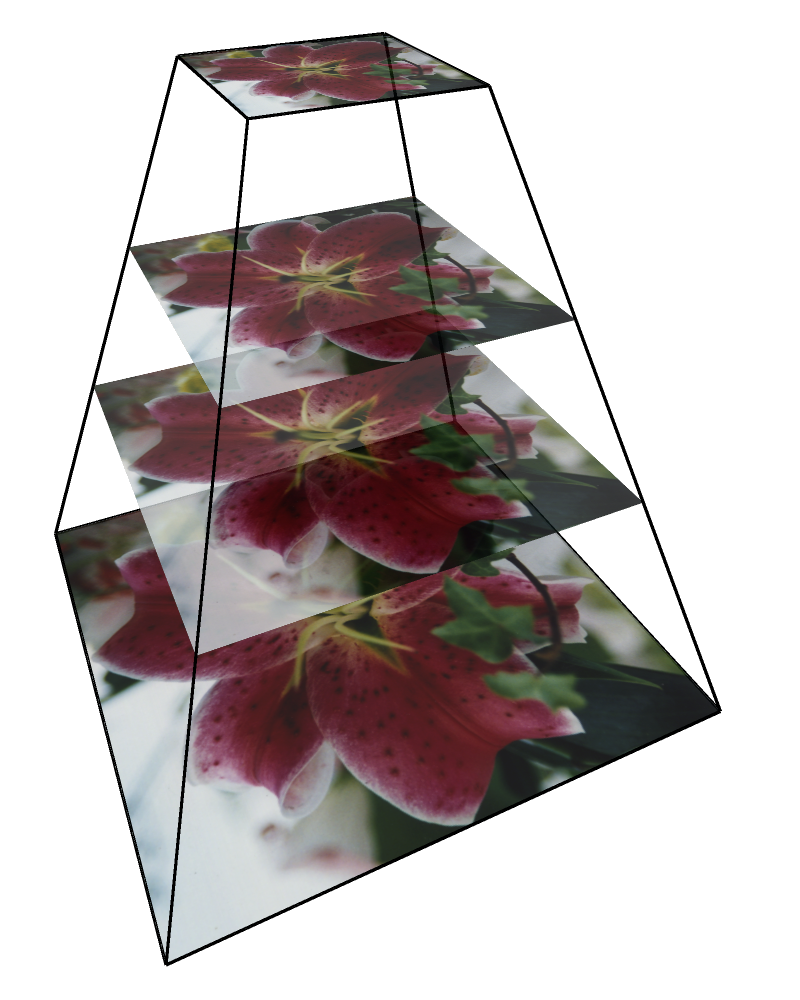
\includegraphics[scale=0.15]{img.png}}
		\subfloat[Calcul des minimums dans la pyramide d'échelle de l'opérateur DoG]{
			\begin{tikzpicture}[scale=.6]
				\draw [<-, > = angle 90, line width=0.3mm, black] (-4, 8) -- (-4, 3);
				\node[align=left] at (-2.75,7.75) {échelle};
				\begin{scope}[yslant=0.5, xslant=-1]
					\fill[step=5mm, blue] (2,1.5) rectangle (3.5,3);
					\draw[step=5mm, black] (1,1) grid (4,4);
					\draw[step=5mm, thick, black] (1,1) rectangle (4,4);
				\end{scope}
				\begin{scope}[yshift=50, yslant=0.5, xslant=-1]
					\fill[step=5mm, white] (1,1) rectangle (4,4);
					\fill[step=5mm, blue] (2,1.5) rectangle (3.5,3);
					\fill[step=5mm, red] (2.5,2) rectangle (3,2.5);
					\draw[step=5mm, black] (1,1) grid (4,4);
					\draw[step=5mm, thick, black] (1,1) rectangle (4,4);
				\end{scope}
				\begin{scope}[yshift=100, yslant=0.5, xslant=-1]
					\fill[step=5mm, white] (1,1) rectangle (4,4);
					\fill[step=5mm, blue] (2,1.5) rectangle (3.5,3);
					\draw[step=5mm, black] (1,1) grid (4,4);
					\draw[step=5mm, thick, black] (1,1) rectangle (4,4);
				\end{scope}
				\end{tikzpicture}
		}
		\caption{Utilisation de la pyramide d'image}
	\end{figure}
\end{frame}

\begin{frame}
	contexte et presentation du parc 

	Première mise en evidence et quantification de la transformation du paysage.

	\begin{figure}
	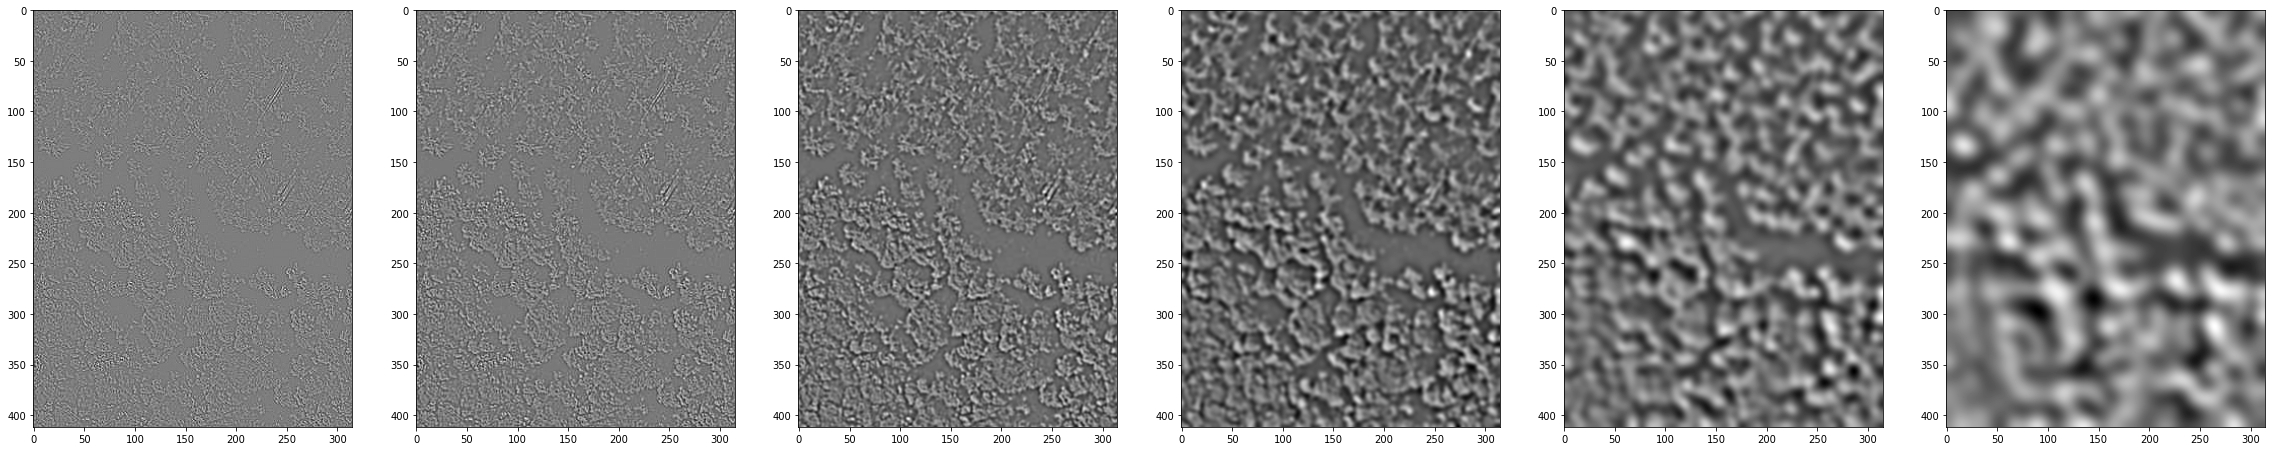
\includegraphics[scale=0.15]{index.png}
	\caption{Pyramide d'échelle de l'opérateur LoG grossière ( 6 octaves sans intervalle ). Image originale \copyright IGN, 2021  }
	\end{figure}
\end{frame}

\begin{frame}
	\begin{figure}
		\subfloat[Agencement désordoné de feuillus, \copyright IGN, 2021]{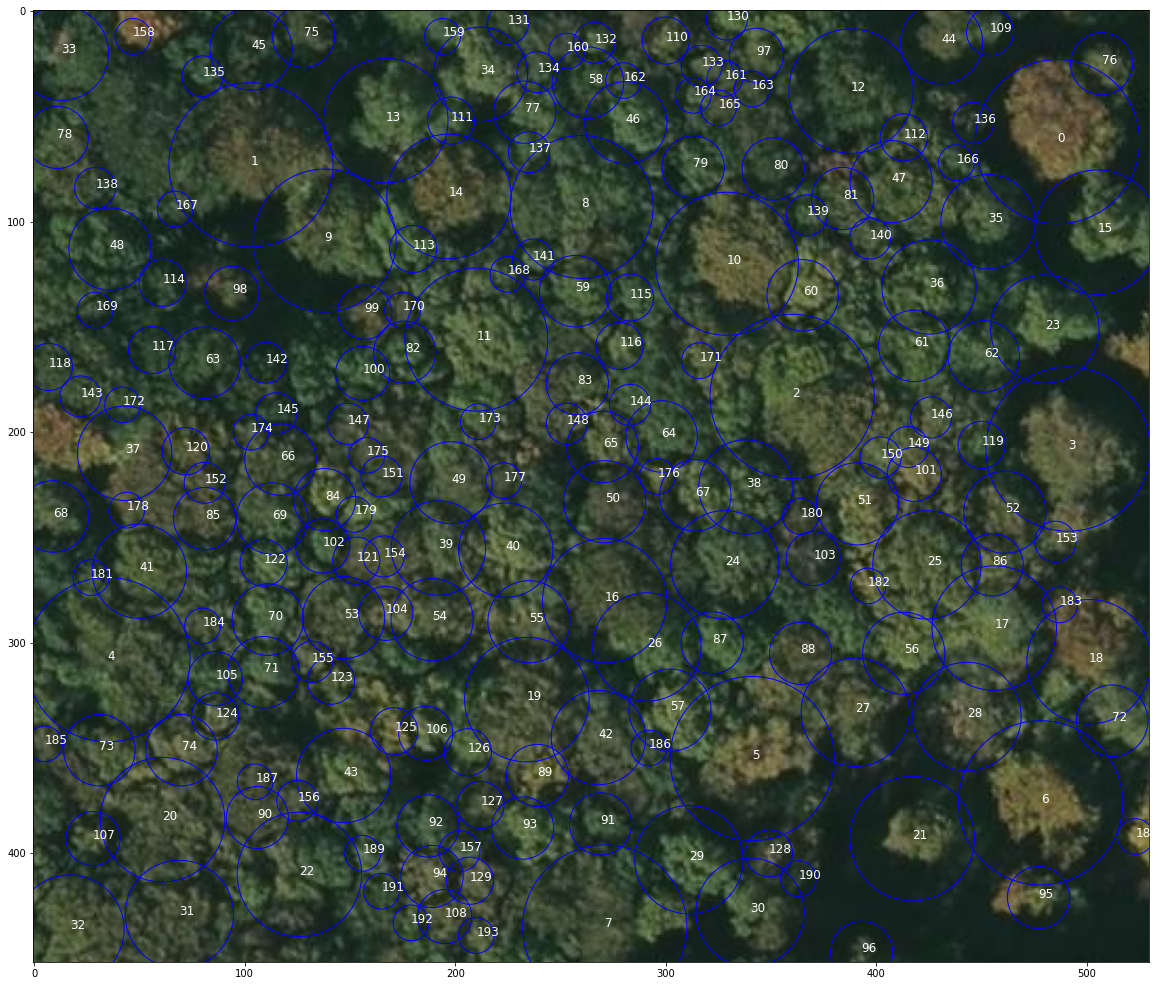
\includegraphics[scale=0.14]{res1.png}}
		\subfloat[Feuillus désordonnés et dougals semi-ordonné, \copyright IGN, 2021]{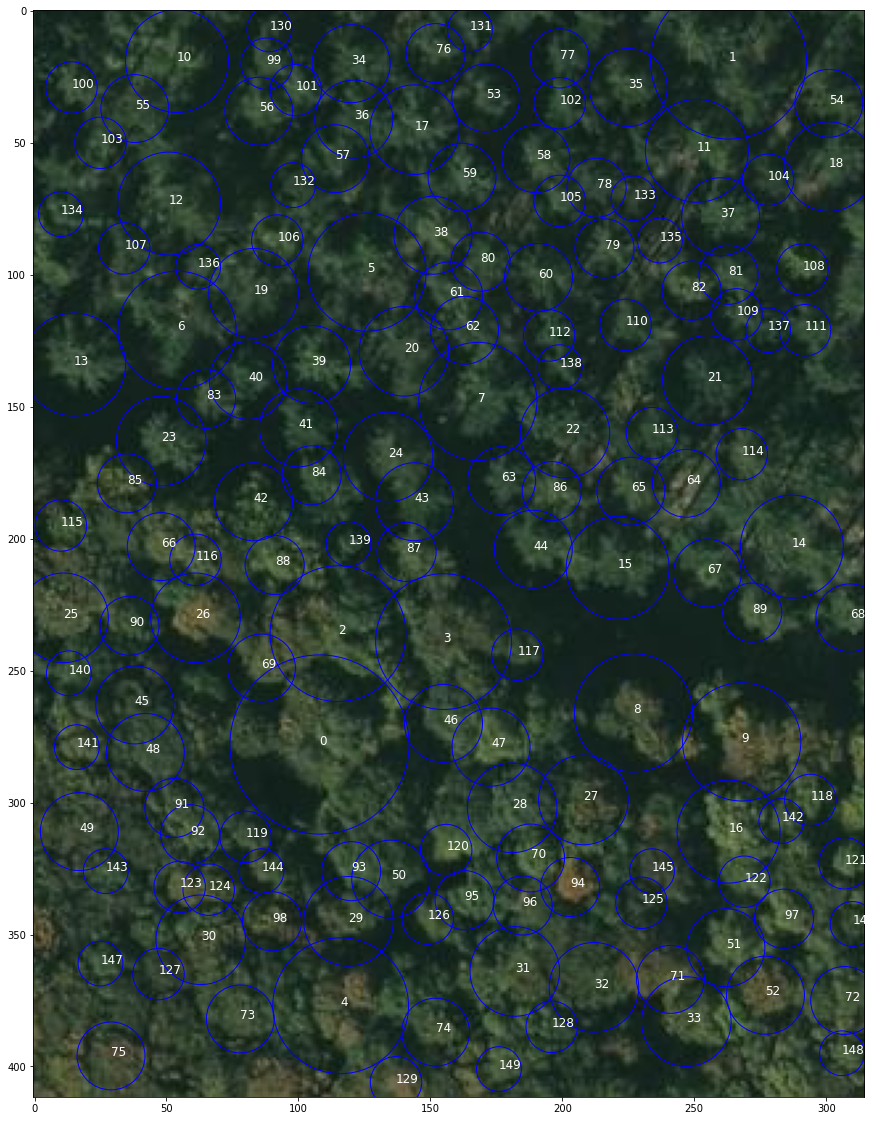
\includegraphics[scale=0.14]{res2.png}} %TODO!!!
		\caption{Résultats obtenus pour 5 octaves, 5 intervalles et $\sigma=0.5$}
	\end{figure}
\end{frame}


\section{Identification des espèces}

\begin{frame}
	
\end{frame}

\section{\'{E}valuation des résultats et prolongements envisageables}

\begin{frame}
	tableau detection pour chaque espèce et resultat d'autres papiers 
\end{frame}

\begin{frame}
	Différents prolongement sont envisagables: 
	\begin{enumerate}
	\item Sensible aux ... séparer préalablement et éventuellement grossiemerement les zones forêstières des zones d'habitation ou  industrielle. Même une route bétonné peut éventuellement altérer les réusltats. batiement/contruction quo fausserait les resultat. 
	De plus obtient qu'un cercle autour des arbres
	\item une methode watershed segmentation avec marqueurs que l'on à trouvé pourrait etre envisagble pour delinéer parfaitement les arbres (voir papier) 
	\end{enumerate}
\end{frame}

\end{document}

